% !TeX program = xelatex
% 在 docs/latex/ai-authoring 目录运行两次 xelatex creator-platform.tex。
% 单文件源码，图由 TikZ 绘制。发布的 PDF 位于 output/pdf/Redflag-AI-Creator-Platform.pdf。
\documentclass[UTF8,11pt,fontset=fandol,a4paper]{ctexart}
\usepackage[top=21mm,bottom=21mm,left=22mm,right=22mm]{geometry}
\usepackage{tikz,tabularx,array,booktabs,fancyhdr,hyperref,xcolor,verbatim}
\usetikzlibrary{arrows.meta,positioning,calc}
\definecolor{ink}{HTML}{172F3B}\definecolor{teal}{HTML}{14675D}
\definecolor{muted}{HTML}{425D67}\definecolor{pale}{HTML}{EBF4EF}
\definecolor{sea}{HTML}{EAF0F5}\definecolor{gold}{HTML}{F8F1E2}
\hypersetup{colorlinks=true,linkcolor=teal,urlcolor=teal,filecolor=teal,pdftitle={Redflag 开发者方案：用候选库与行为树创作 LLM 玩法},pdfauthor={Redflag 项目设计}}
\ctexset{section={format=\Large\bfseries\color{ink},afterindent=true},subsection={format=\large\bfseries\color{teal},afterindent=true,beforeskip=.65\baselineskip,afterskip=.1\baselineskip}}
\pagestyle{fancy}\fancyhf{}\lhead{\small Redflag\quad 开发者方案}\rhead{\small LLM 玩法创作\quad 2026.11.22}\rfoot{\small\thepage}
\setlength{\headheight}{15pt}\setlength{\parindent}{2\ccwd}\setlength{\parskip}{.38\baselineskip}\setlength{\emergencystretch}{5em}
\setlength{\tabcolsep}{4pt}\renewcommand{\arraystretch}{1.28}
\newcolumntype{Y}{>{\raggedright\arraybackslash}X}
\newcolumntype{L}[1]{>{\raggedright\arraybackslash}p{#1}}
\newcommand{\pg}[1]{\clearpage\section{#1}}
\newcommand{\f}[1]{\texttt{\detokenize{#1}}}
\newcommand{\src}[2]{\href{#1}{#2}}
\newcommand{\figcap}[1]{\par{\small\color{muted}\noindent #1\par}}
\tikzset{card/.style={rounded corners=2pt,draw=teal!55,fill=white,text=ink,align=center,font=\small,minimum height=10mm},
  flow/.style={-{Stealth[length=2mm]},line width=.8pt,draw=teal},
  band/.style={anchor=west,font=\small\bfseries,text=ink}}
\begin{document}
\section*{一次真实的试玩与修改}
维修间里，玩家需要走到橙色阀门旁，按 E 打开它。我们在项目副本中将行走速度改为零，又把 HUD 提示缩为 12 像素。模型从正式 Vulkan 游戏的画面和每帧的角色状态选择操作。第一局游戏收到了前进键，记录中的角色位移始终是零。开发者指定的速度是每秒 2 米，字号是 26 像素。模型将这两个值写进同一次修改，前者保存在场景，后者保存在布局。

\begin{center}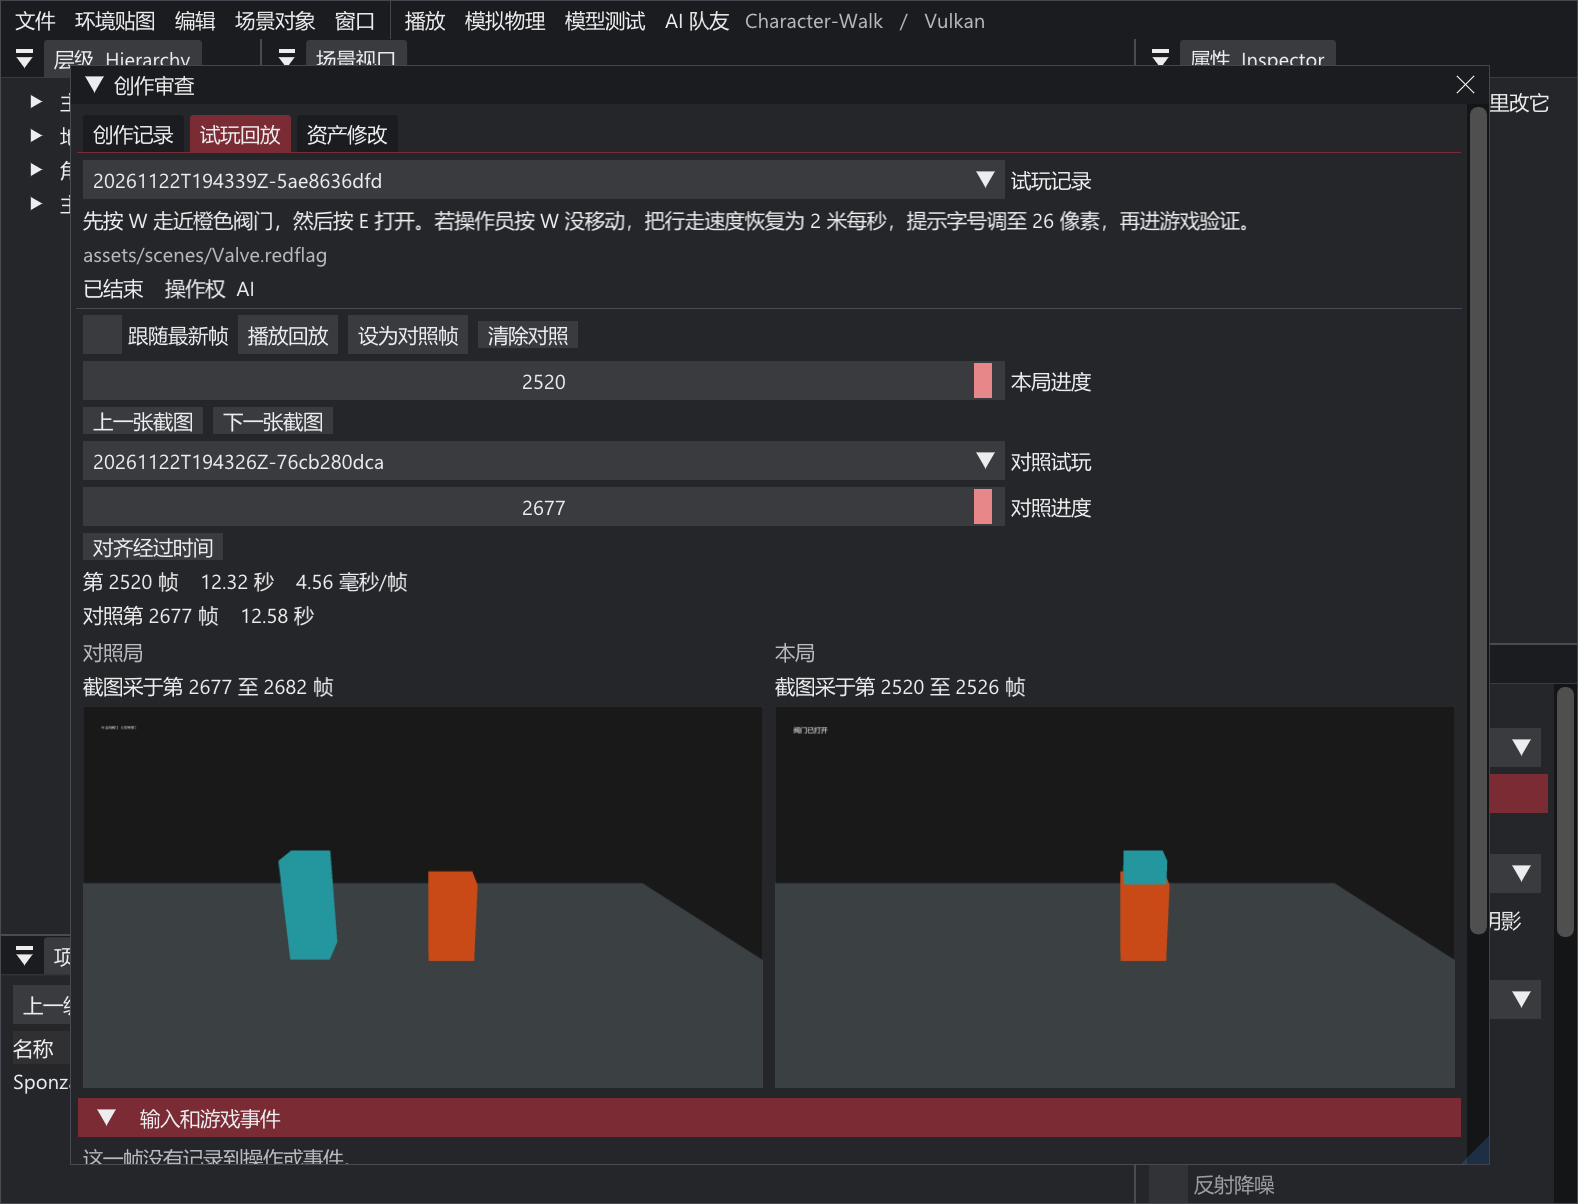
\includegraphics[width=\linewidth]{../../../output/validation/creation-review/forge-playtest.png}\end{center}
\figcap{Forge 实机。左图中操作员停在起点，右图中角色已走到橙色阀门旁，屏幕提示阀门已经打开。图片采集前后的游戏帧号写在各自画面上方。}

第二局里，角色移动了 1.25 米，进入操作范围。随后模型按下 E，游戏脚本确认阀门打开。到达后模型还多按了两次 W，人可以点回这几帧，看这段停顿是否自然。需要接管时，Forge 将控制权交给开发者，游戏松开模型按住的键。选择一个实体和帧号即可留下意见。

在“资产修改”页撤销此次操作，行走速度和字号会一同恢复。作者同时写在别处的设置仍被保留。如果作者改动的正好是模型要调的字号，工具会指出当前值，等作者作出取舍。完整操作和输入、事件、录音的接入方法见 \src{run:../../docs/Playtest-Harness.md}{试玩与修订手册}。以下章节继续讨论原先的玩法创作设计，其中标为拟议的面板按设计方案阅读。
\clearpage
\section{在 Forge 里做一个失物招领处}
创作者输入一句话：「做一个夜班失物招领处，阿榆帮玩家找缠蓝胶带的工具盒；看不清就问，交还以后才结案。」希望得到的结果是能按下“运行游戏”试玩的关卡。之后作者可以双击阿榆的动作、打开剧情结点、改一句提示，或者用 C\# 给关卡加条新规则。下面的面板、接口和示例均为拟议设计。第 2 节单独列出仓库已有的入口。

\subsection*{创作者从哪里动手}
打开项目设置里的“模型连接”，选自己部署的服务或兼容的远程服务，给连接起名“剧情导演”，点“试发”。在项目资源中新建剧情“夜班招领”，把角色表拖到导入窗口。场景中创建“阿榆”，在属性面板选择角色表的一行、模型连接，以及允许它读取的场景信息。没有美术模型时也能用代用角色和两个盒子测试整条玩法。

打开“候选库”，搜索“指向”“追问”“交还”，把三张卡拖给阿榆。双击“交还”打开复用的行为树，绑定目标端口和交接动作。打开剧情图，把“已交还”连接到“结案”。点击试玩，说“找蓝胶带的那只”。此时可以在同一画面看到角色、亮起的行为树分支、模型收到的候选和等待触发的剧情条件。

\subsection*{一句话生成之后，作者还能接手}
这句话可以交给编辑助手，也可以按上述步骤亲自做。助手先查询当前构建支持的编辑命令、资源类型、脚本动作和已安装服务，再搜索项目候选库，列出可复用的树、差的素材和将写入的资产。已有的能力走编辑命令生成可撤销的改动；缺一个项目规则时创建 C\# 脚本并编译；只有底层能力确实缺失、作者已允许改引擎时才修改对应源码，再重建、刷新能力清单。助手读回场景、验证引用、启动同一条试玩流程；只有试玩验证通过才能报告生成成功。

假设作者中途把“自动交还”改成了“先问玩家”。编辑器保存时更新该资产修订号；脚本或源文件被外部编辑后，重新读入并更新修订。助手提交补丁前比较基准版本，只重读受影响的图、字段和连接，保留作者的新分支。两方改了同一条边时，面板列出双方改法让作者选择。下一轮试玩显示实际加载的脚本和图版本。

\figcap{阅读顺序\quad 第 2–4 节对照 Delivery、UE 与 Redflag，给出 Runtime AI SDK 的最短落地路径。第 5–7 节讲候选库、行为树和剧情，第 8–9 节讲 C\# 和流式语音，最后两节给出技术选型和验收方法。}

\pg{Delivery 哪些做法能搬到 Redflag}

Delivery 的\src{run:D:/Udev/Delivery/Document/Diagrams/AI/overview.svg}{系统类图}画出一轮交互中谁有决定权，\src{run:D:/Udev/Delivery/Document/Diagrams/AI/stream.svg}{流式时序图}画出对白与声音何时到达。把两张图放在一起看，创作者会遇到两个不同的问题：一句话可不可以立刻显示，以及角色能否执行这句话里提到的事情。

\subsection*{角色档案、这次能选的动作和实际执行}

Delivery 的人物档案有 JSON 源文件，游戏使用 UE 数据表。\src{run:D:/Udev/Delivery/Source/Delivery/AI/Characters/DeliveryNpcProfile.h}{人物表的行结构}声明姓名、性格、声音及行为表现。另一份\src{run:D:/Udev/Delivery/Design/AI/NpcBehaviorCatalog.json}{行为目录}记录动作、分类、显示名和描述，\src{run:D:/Udev/Delivery/Source/Delivery/AI/Decision/DeliveryNpcBehaviorCatalog.cpp}{候选过滤函数}还会按角色和玩家请求筛选。决策组件在 \f{BuildDecisionRequest} 中把动作、目标编号和证据配成候选项。模型选出一项后，游戏服务器在 \f{TryAcceptProposal} 核对请求、世界与计划版本，行为树任务才开始移动或转向。说话对象可以与动作目标不同，例如店员面向货架找货，同时回答身后的玩家。见\src{run:D:/Udev/Delivery/Source/Delivery/AI/Decision/DeliveryNpcAgentComponent.cpp}{决策组件}与\src{run:D:/Udev/Delivery/Document/Diagrams/AI/behavior.svg}{行为树图}。

\subsection*{网关留下请求的归属，脚本决定用途}

Delivery 的\src{run:D:/Udev/Delivery/Source/Delivery/AI/Network/DeliveryAiGatewaySubsystem.cpp}{网关}接收角色的决策请求，逐行派发回复，在游戏线程处理取消和超时。\src{run:D:/Udev/Delivery/Tools/DeliveryAI/streaming.py}{Python 后端}分别发出模型完成、语音分块及后台工作完成事件。玩家是否已经听完一句话，还要看本机播放器。Redflag 可沿用请求编号和这些事件的含义，把调用者扩大到 C\# 脚本和编辑器工具。人物 CSV 由项目导入，某个选项接哪棵树、哪次行动改变剧情，也由创作者在资产里绑定。玩家插话可以停掉尚未播放的声音，让店员继续找货；若玩家明确说“算了”，游戏才根据自己的规则结束找货任务。这条区别在 Delivery 的\src{run:D:/Udev/Delivery/Source/Delivery/AI/Tests/Conversation/DeliveryNpcPlayerInterruptionTests.cpp}{打断测试}里有对照：检查打断前后的活动编号、目标、开始时间和执行时限。

Redflag 已有 Mono 脚本生命周期。\src{run:D:/Cdev/Redflag/RedflagForge/src/ForgeLayer.cpp}{OpenGL 编辑器}进入 Play 会启动脚本；\src{run:D:/Cdev/Redflag/RedflagForge/src/VulkanForgeLayer.cpp}{Vulkan 编辑器}目前复制场景进入模拟，更新物理与动画。要让两个窗口里的脚本都能收到模型回复，Vulkan 还需接入同一套 Play 生命周期。现有\src{run:D:/Cdev/Redflag/Redflag/src/Redflag/Scene/NpcVision.h}{识图入口}返回候选实体或相机看向的区域，后者只有方向。作者可以拿它给角色指路；若要拿起实物，脚本再按当前实体、手距和遮挡调用拿取检查。一个只靠文字做谜题的项目可以跳过整段识图流程。

\pg{项目资源、游戏世界与模型服务}
把阿榆放进场景时，场景保存角色配置的引用。同一份“交还工具盒”可以由两个角色共用。各角色在游戏实例中分别持有当前目标、正在运行的树节点和自己的请求。Forge 只订阅选中实例的调试事件。停止试玩会释放实例与请求，项目里的树仍可编辑。

\begin{center}
\begin{tikzpicture}[x=1cm,y=1cm]
\draw[rounded corners=3pt,draw=muted!60] (0,0) rectangle (15.6,-6.98);
\fill[pale] (.1,-.1) rectangle (15.5,-2.12);
\fill[sea] (.1,-2.23) rectangle (15.5,-4.43);
\fill[gold] (.1,-4.54) rectangle (15.5,-6.87);
\node[band] at (.3,-.38){创作时\quad 编辑命令读写带版本的项目资源};
\node[card,text width=3.7cm](editor) at (2.45,-1.35){Forge 面板、C\# 编辑工具\\候选库、行为树、剧情图};
\node[card,text width=3.6cm](cmd) at (7.8,-1.35){编辑命令\\检查、预览、采用、撤销};
\node[card,text width=3.8cm](asset) at (13.0,-1.35){项目资产与稳定引用\\角色表、树、剧情、服务配置};
\node[band] at (.3,-2.56){运行时\quad 游戏脚本决定提供的上下文和可以执行的动作};
\node[card,text width=3.7cm](world) at (2.45,-3.55){游戏世界与剧情存档\\动作生效后发出事件};
\node[card,text width=3.6cm](tree) at (7.8,-3.55){行为树、剧情实例\\C\# 动作与对话};
\node[card,text width=3.8cm](ctx) at (13.0,-3.55){读取角色配置和候选\\组装本次请求};
\node[band] at (.3,-4.90){异步服务\quad 网关安排请求，后端调用模型或本地推理进程};
\node[card,text width=3.7cm](model) at (2.45,-5.97){可选模型与音频服务\\LLM、VLM、STT、TTS};
\node[card,text width=3.6cm](backend) at (7.8,-5.97){AI 后端\\供应商适配、流式输出};
\node[card,text width=3.8cm](gate) at (13.0,-5.97){引擎 AI 网关\\排队、取消、主线程派送};
\draw[flow](editor)--(cmd);\draw[flow](cmd)--(asset);
\draw[flow](asset)--(ctx);\draw[flow](ctx)--(gate);
\draw[flow,<->](ctx)--(tree);\draw[flow,<->](tree)--(world);
\draw[flow,<->](gate)--(backend);\draw[flow,<->](backend)--(model);
\draw[flow,dashed] (gate.north west)--(tree.south east);
\end{tikzpicture}
\end{center}
\figcap{图 1\quad Redflag 拟议架构（项目原创）。单箭头表示写入、读取或发起调用，双箭头表示请求与回执。虚线是网关把模型事件交回实例。联网时主机持有能改变共享世界的实例。}

扩展现有 \f{AssetLibrary} 的资产类型。角色档案、能力集合、行为树、剧情、模型连接能在项目窗口中搜索，也能从引用跳回原文件。树节点消费带类型的参数，连接只保存稳定 ID。模型连接记录地址、能力和鉴权引用；发布的联网游戏由服务端持有供应商密钥。C++ 负责主线程和世界对象，创作者用 C\# 或面板，部署方可以独立维护 Python 后端。

“模型连接”要显示试连的结果和已验证能力，例如文本、图片、结构化选择、语音流。项目只装文本服务时，创作者就能完成谜题、旁白与剧情。选择需要视觉或语音的节点时，属性面板提示具体缺哪项服务，并能跳到配置。

工程命名建议用 \f{Redflag.AI}（运行时公开 SDK）、\f{Redflag.Editor.AI}（Forge 扩展）和“Redflag AI 后端”（独立服务）。在项目内用带版本号的 YAML 保存创作图、候选定义和连接配置，CSV 保存静态档案，已有场景继续用原格式引用资产。打包时把这些源文件编译成运行时读取的定义。协议、资产格式各自有版本；编辑器、C\# 和运行游戏用同一批动作 ID 和表定义。UE／Delivery 作为行为与协议的参考宿主，首个原生实现落在 Redflag。

\pg{借 UE 的模块边界，做轻量 Runtime AI SDK}
项目可将它称为 \textbf{Redflag AI Runtime SDK}。随游戏发布的部分负责连接、请求和事件；Forge 工具用同一个 SDK 试跑和订阅。可先在现有 C++ 工程里按目录和依赖隔开，C\# 外观放进现有脚本程序集，编辑器扩展另放 Forge。这样第一条链就能验证这套 SDK，将来决定是否单独发布二进制包也有清楚的边界。UE 的 Runtime／Editor 模块与随游戏实例释放的子系统适合作为参考。\src{https://dev.epicgames.com/documentation/en-us/unreal-engine/unreal-engine-modules}{Epic 模块说明}；\src{https://dev.epicgames.com/documentation/en-us/unreal-engine/programming-subsystems-in-unreal-engine}{Epic 子系统生命周期}

\begin{center}\small
\begin{tabularx}{\linewidth}{@{}L{27mm}Y Y@{}}\toprule
拟议边界 & 公开给谁、谁来持有 & 为什么能更快做出玩法 \\ \midrule
运行时 SDK & C++ 游戏宿主持有网关；C\# 和图节点共享“发请求、收事件、取消”。每次试玩有独立会话，场景与脚本各自拥有其请求。 & 文本终端和角色都能调用。发布游戏或无界面的主机能独立运行；停止一次试玩能准确清掉它的请求。\\
Forge 创作工具 & 面板只持当前选择、草稿和调试订阅。候选库、模型试发和自定义工具共用项目资产与 SDK。 & 先用表格、下拉框、树列表和日志做通；连线画布随后读取相同的节点与连接数据。\\
AI 后端和扩展 & 自有后端对上游做模型适配，接收启动和取消。WebRTC 插件处理媒体，动作与故事插件按项目选用。 & 第一条链只需要一个文本提供器。增加一个 VLM 或改声音时，已有剧情、动作脚本和场景可原样使用。\\ \bottomrule
\end{tabularx}
\end{center}

\subsection*{最短的一条接通路径}
选一个可访问的文本模型端点，在自有后端写一个适配器，把上游流转换成统一的文本增量、完成、错误事件。Delivery 的 \f{stream_api} 已有读取兼容服务 SSE 的示例；其对外 \f{/v1/decisions/stream} 收 NPC 专用数据。Redflag 可以复用它配置的上游模型服务和解析经验，自行定义通用请求。随后从 Forge 和一个游戏脚本分别调用同一入口，测试取消、重进和发布运行。第二步把一个有类型的候选选择绑定到现成动作；这样无需等语音、画布或 3DGS 就能交互。\src{run:D:/Udev/Delivery/Tools/DeliveryAI/streaming.py}{Delivery 流读取代码}；\src{run:D:/Udev/Delivery/Tools/DeliveryAI/server.py}{Delivery HTTP 路由}

角色组件只保存模型配置、可读场景和技能集的引用，角色所持的树负责执行。通用请求也可由菜单、剧情导演或编辑器发出。Convai 的 UE 会话设计把共享媒体连接与角色、玩家组件的启停分开。NVIDIA ACE 的 UE5 插件让开发者从 Blueprint 或 C++ 使用识别、语言模型与合成。Redflag 可借这两处设计，让面板、图节点和 C\# 共用操作，只初始化项目选用的服务。\src{https://github.com/Conv-AI/Convai-Documentation/blob/main/plugins-and-integrations/convai-unreal-engine-plugin/core-concepts/session-lifecycle.md}{Convai 会话生命周期}；\src{https://developer.nvidia.com/blog/build-on-device-ai-companions-with-the-nvidia-ace-game-agent-sdk-and-unreal-engine-5-plugins/}{NVIDIA ACE SDK 与 UE5 插件}

\pg{一个能编辑、试选和追踪的候选库}
项目有“可以怎么做”的资源；每轮游戏另有“此时能对谁做”的实例。打开候选库默认看到作者维护的动作、可复用子树、对话意图和剧情片段。切到“调试当前轮”，选择阿榆和刚才那句话，就能看到本轮生成的目标和证据。物件可以没有公开名称；图片里的陌生目标也能出现在这里。

\begin{center}\small
\begin{tabularx}{\linewidth}{@{}L{24mm}YY@{}}\toprule
作者看到的分类 & 创作时可以改什么 & 试玩时可以查什么 \\ \midrule
动作与子树 & 新建“交还物品”，设置说明、目标端口、适用角色和执行子树；可另绑 C\#。 & 项目有这张卡，阿榆已装备；尚未确认目标，暂不能提交交接。\\
目标与证据 & 选择目标提供器、公开字段、视角或查询范围；可放一份样例观察试选。 & 点“柜台右侧”打开拍摄时的图、区域和时间；若已关联实体，可另看它现在的位置。\\
意图与剧情 & 新建“澄清特征”“归还失物”，填触发条件、所需事实和允许的下一步。 & 能查到追问选项发给了模型；“结案”因缺少交接回执被排除。\\
服务与资源 & 从项目资源挑模型连接、音色、姿态或动画片段，试听、预览并检查引用。 & 显示此轮的模型、语音连接和树实际播放的动画，可打开源资产。\\ \bottomrule
\end{tabularx}
\end{center}

\subsection*{选中“交还物品”时，检查器应该显示什么}
卡片有稳定动作 ID、作者可改的显示名、给模型读的一句话、参数类型、可用条件、执行入口和结果。作者可搜索、复制、拖入角色、打开关联树、用样例输入单独运行。编辑给模型的描述可以看下一次请求的变化；修改公共卡时可查看引用它的角色。能改变世界的卡应明确谁来确认成功，例如“玩家实际收到同一件物品”。

运行时按“项目全部 → 角色启用 → 条件通过 → 本轮发出 → 模型选中 → 执行结果”逐步显示。点灰色项看首个失败条件；点未入选项可区分“超出候选上限”和“已发给模型、模型选了别项”。数量多时先按角色能力、剧情条件和目标范围过滤；检索器若做排序，可显示它自己的分数和截取位置。面板只显示确实记录过的输入、筛选规则、输出和回执。

例如卡“指向”可接图片区域或实体，卡“交还”要求可交互实体。旧图上的蓝盒只有一块区域时，前者仍可入选，后者显示“目标端口缺实体”。给模型的是本轮临时选项号及可读描述。引擎保存选项号对应的动作、目标、证据和修订；模型交回选项号后再校验当前世界。候选列表并不要求开发者逐件给场景物体登记名字。

\pg{让上层 AI 节点接入可展开的行为树}
在图上创建“从候选中选择”，把候选卡拖到输出端口，再把每个端口接到一个子树资源。节点在玩家开口、任务阶段改变或上一步有必要重新选择时拍下输入，发一次请求，等待时显示“运行中”。作者可以直接点进正在执行的那棵树看停在哪一步。等待移动、等玩家回答和播放动画都由游戏时间推进。

\begin{center}
\begin{tikzpicture}[x=1cm,y=1cm]
\draw[rounded corners=3pt,draw=muted!60] (0,0) rectangle (15.6,-5.52);
\fill[pale] (.1,-.1) rectangle (15.5,-2.12);
\fill[sea] (.1,-2.22) rectangle (15.5,-5.42);
\node[band] at (.3,-.41){阿榆的决策图\quad 点击输入可以查看这一轮的证据};
\node[card,text width=3.2cm](event) at (2.25,-1.36){玩家问询\\或执行失败};
\node[card,text width=3.7cm](choose) at (7.80,-1.36){从候选中选择\\输入含动作、目标与观察};
\node[card,text width=3.2cm](miss) at (13.30,-1.36){未匹配或连接超时\\使用作者写的默认回应};
\draw[flow](event)--(choose);\draw[flow](choose)--(miss);
\node[card,text width=3.5cm](ask) at (2.6,-3.50){追问子树\\说明疑点，等玩家回答};
\node[card,text width=3.5cm](point) at (7.80,-3.50){指向子树\\转身，指向候选区域};
\node[card,text width=3.5cm](give) at (13.00,-3.50){交还子树\\走近，复核，递交};
\draw[flow](choose.south)--++(0,-.51)-|(ask.north);
\draw[flow](choose.south)--(point.north);
\draw[flow](choose.south)--++(0,-.51)-|(give.north);
\node[font=\small,text=muted] at (7.8,-4.89){双击“交还”可查看目标端口、当前步骤、动画和世界回执。};
\end{tikzpicture}
\end{center}
\figcap{图 2\quad 原创拟议编辑器视图。连线由作者保存，每轮只高亮实际走过的边；等待、成功、失败、中止都有文字状态。}

选择“场景信息”时，提供器返回作者放行的字段、观察时刻和引用。“全场任务状态”适合剧情导演；阿榆可以选“角色视野内的实体”。选择“3DGS 图片”时，先从离线重建场景取相关站位的图，再让视觉模型返回区域或实体候选。两种来源可独立用，也可并列显示。原始 3DGS 论文解决从照片重建并绘制新视角；识别、找实体和拿取分别交给视觉模型、场景查询和角色动作。\src{https://repo-sam.inria.fr/fungraph/3d-gaussian-splatting/}{Kerbl 等，SIGGRAPH 2023}

执行失败时把真实原因传回图。例如另一个玩家拿走了盒子，当前子树给出“目标已易手”，作者可接“告知玩家”或“再观察一次”。等待中的节点中止时撤销请求，已完成的交接保留。语言层选技能、执行结果再进入下次决策，可以对照机器人论文的两个独立实验思路。编辑器运行树可借鉴 LimboAI 按实例查看任务和黑板的操作。\src{https://say-can.github.io/}{SayCan}；\src{https://innermonologue.github.io/}{Inner Monologue}；\src{https://limboai.readthedocs.io/en/stable/behavior-trees/create-tree.html}{LimboAI 作者手册}

\pg{剧情作者怎样控制事实与对白}

玩家来到失物招领处，说“我来拿蓝胶带的工具盒”。创作者希望阿榆记得玩家描述过什么，也希望他亲自查找，拿错时还能改口。作者可以把这段故事分成“登记”“查找”“待认领”“已交还”四个节点，为每个节点填写进入条件、此刻允许的选项和离开后发生的事件。想让阿榆说话更活泼，可以调整角色表。想让他也能请同事帮忙，就在“查找”节点加一个选项。

\subsection*{阿榆在这一轮知道什么}

在“登记”节点，脚本把角色表里的说话习惯、玩家这句话、已经说过的线索，以及当前允许的“追问特征”和“开始查找”发给模型。假如作者把失主身份写在结局里，组装这轮请求时就只读取当前节点公开的字段。模型可以说“蓝胶带缠在提手上，还是贴在盖子上？”，再提议“追问特征”。玩家答“提手上”后，游戏把它记为玩家提供的线索。以后玩家改口说“是盖子”，旧话仍可查，下一轮查找采用更新后的描述。

\subsection*{谁来确认盒子已经交还}

模型提议“开始查找”，脚本核对当前节点和选项，把描述交给查找行为树。树能返回“找到候选”“现场已经移走”或“未找到”。找到候选时，阿榆可以指给玩家看，故事进入“待认领”。这时即便台词已经播到“我这就给你”，任务仍在进行。等玩家认领、游戏主机确认盒子已转入玩家持有，再用本次交还的事件编号推进到“已交还”。重复收到同一确认时只记一次。若盒子先被另一位玩家拿走，树返回原因，作者可接回“查找”，让阿榆解释发生了什么。

\subsection*{读档后从哪句话接起}

存档保存当前故事节点、变量、已处理的交还事件编号，以及玩家实际看到的对白。读档时恢复这些记录，回放时直接显示留下的台词。清档重玩则创建新故事实例和对话记忆，再次查找时读取新场景。创作者也能把同一套接口用在终端留言、任务简报或纯文字推理游戏里。

可选用 ink 的 C\# 运行库推进作者分支。脚本读取当下的选项，将模型建议映射到当前有效的选项，并随存档保存 ink 状态。查找行为、交还确认与朗读仍由项目脚本连接。\src{https://github.com/inkle/ink/blob/master/Documentation/RunningYourInk.md}{ink 作者的 C\# 集成与存档说明}

\pg{C\#、CSV 和编辑器扩展怎样配合}
静态人物表导入后生成带类型的行和稳定引用。作者能在表格视图改性格、挑声音，在角色属性里覆盖某一项，也能导出 CSV 用表格软件批量改。约定 UTF-8、列类型和稳定行键；引用列选项目资产，重名键、失效引用精确提示到行列。应用导入前展示差异；校验失败保留上次可用表。项目表的更改写回同一源文件，角色实例的覆盖保存在该角色配置。玩家说过什么、盒子归谁属于存档。

\figcap{拟议示例\quad 项目中的角色源表。模型、音色、能力集是项目内可读的引用键，导入器解析为相应资产的 ID。}
{\small\begin{verbatim}
id,displayName,style,model,voice,skillSet
ayu,阿榆,寡言但会问清细节,director,night_clerk,lost_found
\end{verbatim}
}
\subsection*{游戏脚本按需取文本、图片或候选选择}
纯文本工具只需连接名和消息。运行时把请求绑定到脚本实例；原生网关在工作线程读取字节，游戏线程派送类型化事件。下面是失物招领台脚本的拟议 C\# 伪代码，展示独立的字幕用法。代码中的事件订阅发生在回合开始时；停止试玩、删除所有者或重载脚本时由宿主统一取消并清理订阅。

{\small\begin{verbatim}
void OnPlayerQuestion(string text)
{
    active?.Cancel();
    active = AI.Start(this, "director", AIRequest.Text(text));
    active.TextDelta += subtitle.Append;
    active.Failed += subtitle.ShowError;
}
\end{verbatim}
}

决策节点用同一个 \f{AI.Start}，在请求附上观察与当轮候选，监听完整的选择事件。新动作可以在项目 C\# 中声明稳定动作 ID、参数和处理函数，宿主把描述提供给候选库。举例，“核对取件码”收取玩家输入和当前认领单，返回“相符”或“不符”。脚本编译后它便可搜索、可以接到树上，其他角色也能引用。作者可以给动作绑定现有动画；需要两阶段交接时，用动作回执触发交出帧和持有者切换。

\subsection*{作者也能给 Forge 写自己的工具}
拟议的编辑器程序集 \f{Redflag.Editor} 只在 Forge 加载。作者注册一个菜单“给所选失物起草描述”。点击后读取选择对象和资产修订，仍用 \f{AI.Start} 发请求；面板显示结果，用户点“采用”才用带修订检查的编辑命令修改描述，可一步撤销。接桥可查 \src{run:D:/Cdev/Redflag/Redflag-ScriptCore/Source/Core/InternalCalls.cs}{现有内部调用声明}和 \src{run:D:/Cdev/Redflag/Redflag/src/Redflag/Scripting/ScriptGlue.cpp}{原生注册处}。这些新增 C\# 名称均为设计。

玩家在自己的项目里写 C\#，发布后随游戏运行。如果游戏还允许其他玩家在线上传玩法，可加载受限的“事件、条件、调用已公开动作”规则包。主机按该游戏声明的权限和动作表执行。完整 C\# 扩展按受信任的项目代码发布；现有 Mono 脚本宿主不承担陌生程序集的沙箱职责。

\pg{从玩家开口到游戏收到动作结果}

玩家对阿榆说“把蓝盒子递给……二号窗口的那位”，创作者希望立即出现字幕，阿榆听完再行动。客户端采集声音、绘制字幕、播放回复。引擎网关关联请求与游戏实例，AI 后端持有模型服务的凭据。联网时由推进世界的游戏主机判断交接能否成立，通过游戏网络同步结果。单人试玩时这些部分可以在同一台电脑上运行。

\subsection*{字幕可以逐字出现，交付以游戏回执为准}

文本请求可直接走 HTTP。拟议的网关用 NDJSON 返回事件，每行一个 JSON 对象。一次玩家输入对应一个 \f{turnId}，网关为该轮事件分配递增的 \f{seq}。编辑器和 C\# 脚本可以依次看到转写草稿、正式转写、回复片段、完整动作提议和结束原因。字幕用新草稿替换旧草稿。只有完整提议通过参数检查，创作者绑定的行为树才收到动作。

假设模型提议给二号窗口的玩家递盒子，主机检查盒子的持有者与接收人，执行后按动作编号 \f{actionId} 记录结果。跨连接以会话、回合和请求编号对应事件。断线重连时客户端提交最后收到的事件序号，后端从保留的记录续传。记录已到期就明确结束这一轮。相同动作再次到达时，主机返回原回执。对话系统据此说“交给你了”或“盒子已经被拿走”，并将事实交给剧情脚本。

\subsection*{语音是创作者按需接入的通道}

语音配置选择输入设备、转写服务、声音和回合结束方式。启用远程语音时，WebRTC 传送麦克风和回复音轨。VAD 检测说话与停顿，STT 转写文字，TTS 合成按句发出的回答。“递给”后的停顿可能正在等玩家说出对象。创作者可选松开按键提交，或接入结合上下文的回合判定。玩家插话时，客户端停播旧轮，网关取消后续生成，游戏丢弃旧轮尚未批准的提议。已经递到玩家手里的盒子仍然属于玩家。

可参考 \src{https://docs.livekit.io/agents/logic/turns/}{LiveKit 的回合控制}
和 \src{https://docs.pipecat.ai/pipecat/learn/pipeline}{Pipecat 的流式处理器}。
本地中文转写可试 \src{https://k2-fsa.github.io/sherpa/onnx/pretrained_models/online-paraformer/paraformer-models.html}{sherpa-onnx 的流式 Paraformer}。
编辑器记录玩家结束输入、出现首段字幕、听到首段声音、收到动作回执的时刻。测量时注明模型、机器和网络条件，才能区分慢在识别、生成、播音还是游戏执行。

\pg{可以先试用哪些开源项目}
引擎自己定义项目资产、候选格式、编辑命令和请求事件。下面这些项目各解决一个具体问题。接入前用“阿榆归还盒子”测试哪个值得采用；本次查阅了作者资料，没有在 Redflag 编译、安装或测性能。

\begin{center}\small
\begin{tabularx}{\linewidth}{@{}L{31mm}YY@{}}\toprule
候选项目 & 适合 Redflag 的位置 & 采用前做一个小验证 \\ \midrule
\src{https://github.com/BehaviorTree/BehaviorTree.CPP}{BehaviorTree.CPP} & C++ 行为树执行候选。支持异步任务、类型化端口、子树和状态记录。Forge 可自己画图。 & 启动“走近”后取消，看异步返回会不会唤醒旧实例。以同一份树资产生成运行树，避免维护两套树。\\
\src{https://limboai.readthedocs.io/en/stable/}{LimboAI}／\src{https://github.com/thedmd/imgui-node-editor}{imgui-node-editor} & 前者是 Godot 的创作体验参考；后者是 Dear ImGui 的节点画布候选。可视化和树执行能分别选择。 & 使用 Redflag 当前 ImGui 构建试连带类型的端口，切换两位角色，看各自运行的节点和黑板。\\
\src{https://github.com/inkle/ink}{ink} & 可选 C\# 叙事运行库。故事作者写选项、变量与跳转，项目对接台词、语音和世界事件。 & 编译小故事，存档重进后应处在同一节点，且“交还”只登记一次。\\
\src{https://docs.pipecat.ai/pipecat/learn/pipeline}{Pipecat}／\src{https://github.com/livekit/client-sdk-cpp}{LiveKit C++ SDK} & 前者可承担后端语音处理流程；后者可在原生客户端收发实时音轨。已有后端也能只实现所需适配。 & 用同一句中文测试首段字幕、首声、打断和重连；只让选定的后端协调一次语音回合。\\
\src{https://k2-fsa.github.io/sherpa/onnx/pretrained_models/online-paraformer/paraformer-models.html}{sherpa-onnx} & 本地中文流式识别候选，可与云端 LLM 混用；中文 TTS 也有作者发布的模型。 & 用实际角色名和“蓝胶带”测试错词；在发布机器试听声音，分别核对代码与模型许可。\\
\src{https://github.com/CoplayDev/unity-mcp}{Unity MCP}／\src{https://github.com/anthropics/skills/tree/main/skills/mcp-builder}{mcp-builder} & 前者展示编辑器向外部助手提供工具，后者是编写 MCP 工具的开源技能示例。均作创作端参考。 & Redflag 适配器导出同一组编辑命令；助手能发现、调用、读回，并在碰到作者并发修改时给出差异。\\ \bottomrule
\end{tabularx}
\end{center}

编辑桥可按 MCP 的工具协议公开当前可用命令和参数；资产内容和场景修订另外查询。例如“创建角色”可列出菜单与脚本实现共同调用的命令，读回结果后再挂能力集。让创作者打开同一能力列表，既能看到助手能调用哪些命令，也能查某个插件尚缺什么。模型运行服务和关卡试玩均可在编辑助手离线时独立使用。\src{https://modelcontextprotocol.io/specification/2025-06-18/server/tools}{MCP 工具发现与调用规范（2025-06-18 版）}

\pg{从两条创作入口做到可发布的玩法}
第一里程碑是能在真实场景里玩一次“阿榆归还盒子”。最短链是文字输入、结构化场景、少量作者绑定的动作、宿主复核、持有者改变、剧情收到一次交还回执。用简易列表和执行轨迹即可查原因。下面一、二两项补齐通用接口和候选调试，第三项将这个例子扩展成可编辑的故事与多种观察。后续逐步接好语音、视觉与自动创作。延迟、识别质量、服务费用和支持的角色并发量均待实测。

\begin{center}\small
\begin{tabularx}{\linewidth}{@{}L{28mm}Y Y@{}}\toprule
交付顺序 & 创作者手里的东西 & 可复查的通过条件 \\ \midrule
一、脚本和编辑器接模型 & 项目连接、文本请求、取消，游戏 C\# 样例和自定义编辑工具。 & 空场景做一个文本谜题；两种后端的 Play 都能收回复；工具生成描述后可撤销；停止或重载后无旧回调。\\
二、候选库和可视行为树 & 卡片、能力集、CSV 导入、异步选择、子树、运行检查器。 & 作者新增 C\# 动作并拖入树，不改引擎也能调它；两个角色共享树、目标独立；能看出缺目标、未入选和选择后执行失败的差别。\\
三、剧情和观察 & 接入故事的条件、结果、台词与存档；可独立选择结构化场景或 3DGS 图像。 & 纯文本可通关；用“盒子在／不在／仅旧图有”三种场景测试候选；两个玩家争取同一盒子，只能确认一笔交接。\\
四、语音和发布 & 接入可换的 STT、TTS、VAD 和可选 WebRTC，远程后端与主机权威。 & 在转写、模型输出和播音期间分别插话；丢弃旧轮提议。丢确认后重发，两名观看者的姿态、持有者和剧情节点最终一致。\\
五、一句话创作 & 助手能搜索库、创建项目资产、配树、编译脚本、运行验证；人可中途接管。 & 用首页同一句话生成可玩关卡，再由作者改“必须追问”。助手继续补台词时保留新连接，存盘重开后仍能复现。\\ \bottomrule
\end{tabularx}
\end{center}

验收运行界面时保留三种入口。场景属性能从“阿榆”跳到它引用的卡和树；资产窗口能按名字反查使用这张卡的角色；调试时间线能从迟迟未完成的台词跳回对应回合和树节点。没连真实模型时可用录制回合重放规则、核对实际输入输出；更换模型后再用同一组问题实跑，单独统计候选正确、澄清和误执行的数量。

性能记录同一模型、机器、网络、角色数和样本量，分开测停嘴至首个稳定字幕、至首段可听声音、插话至停播、提议至世界回执的 p50／p95。游戏主线程另测每帧派送耗时。预算超限要能在时间线上分清卡在排队、识别、生成、播音还是行为树。用于联网对照的现成入口是 \src{run:D:/Cdev/Redflag/examples/Network/WorldWorkshop.cpp}{Redflag 主机与观看端示例}；上述 AI 玩法和性能门槛均待实际实现后验证。
\end{document}
